%%%%%%%%%%%%%%%%%%%%%%%%%%%%%%%%%%%%%%%%%%%%%%%%%%%%%%%%%%
%% SLIDE 6: ARCHITECTURE
%%%%%%%%%%%%%%%%%%%%%%%%%%%%%%%%%%%%%%%%%%%%%%%%%%%%%%%%%%

\begin{frame}
    \begin{tikzpicture}[remember picture,overlay]
        \fill[PrimaryBlueLighter, opacity=0.08] ([xshift=-3cm,yshift=2cm]current page.south east) circle (4cm);
        \fill[PrimaryGoldLight, opacity=0.06] ([xshift=4cm,yshift=-2cm]current page.north west) circle (3.5cm);
        \node[anchor=north west, text=FundoQuestion, font=\bfseries\tamanhoQuestion\selectfont]
            at ([xshift=0.8cm,yshift=-0.8cm]current page.north west) {How does eBezout connect everything?};
        \node[anchor=north west, text width=.80\paperwidth, align=left, text=FundoKeyMessage, font=\tamanhoKeyMessage\selectfont]
            at ([xshift=0.8cm,yshift=-1.6cm]current page.north west) {
            A simple AI system connects the product, customer, and supermarket—and turns each interaction into useful information.
        };
    \end{tikzpicture}

    \vspace{0.3cm}
    \begin{center}
        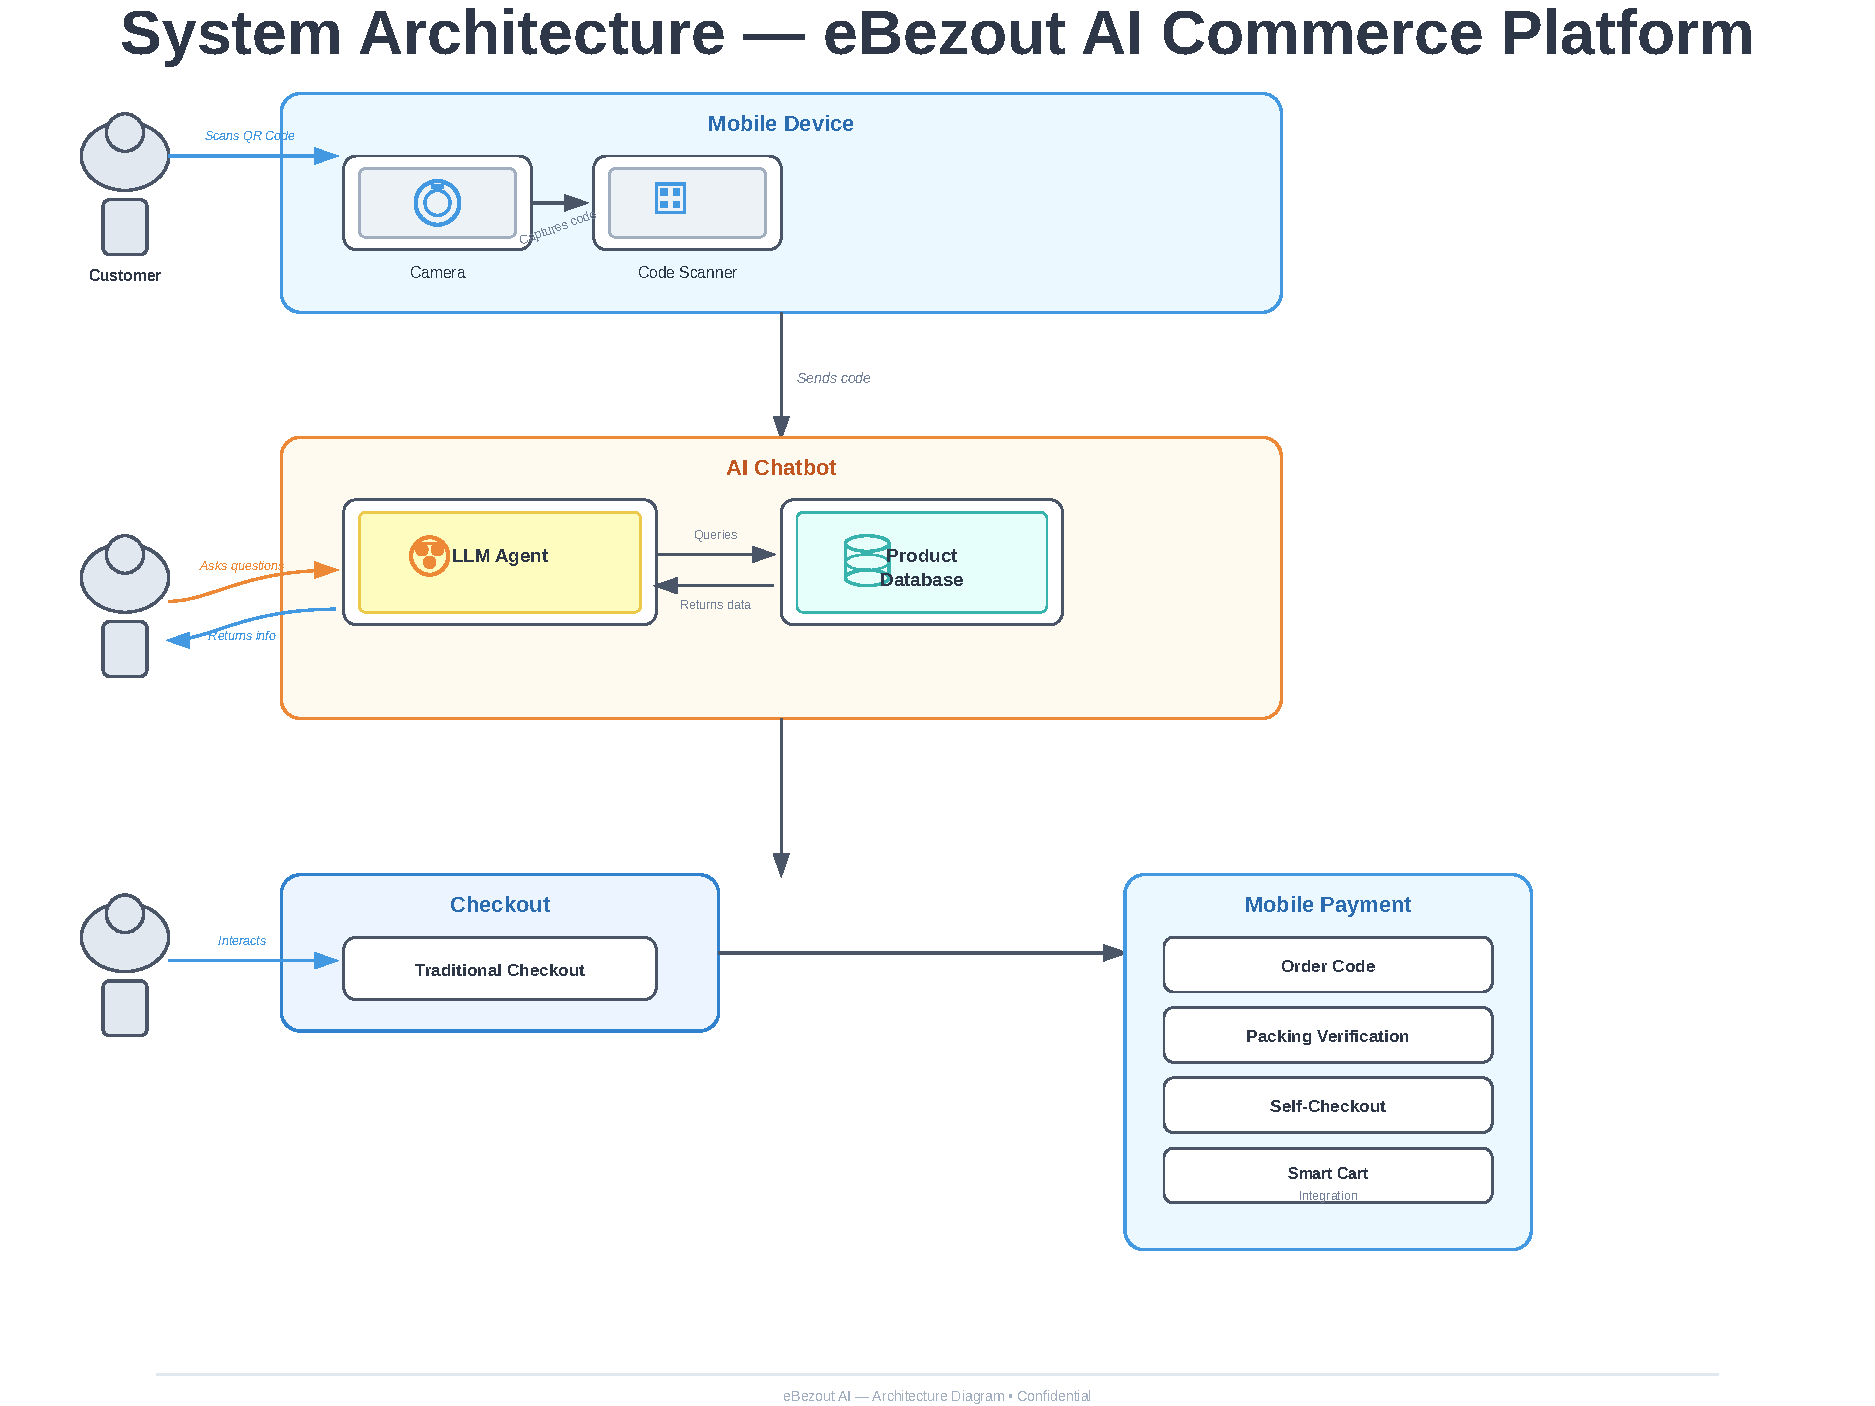
\includegraphics[width=0.80\textwidth]{Images/architecture-diagram.pdf}
    \end{center}

\end{frame}